% VeriCodeGen NeurIPS 2026 research-track submission.
% Main source is usable from the repository root or from submission/.
% Uses the supplied, unmodified workshop style in template/.
% Official template: https://www.overleaf.com/read/fhmwmtrgwkmc
% Compiled PDF is supplied; main-text pagination is checked against 4--9 pages.
% Numerical sources: semantic-diff-test/results/summary.json, graded.json,
% ablation/ablation_summary.json, control_probe/control_probe_summary.json,
% dose_confusable/dose_summary.json, and oracle/data/matrix_meta.json.
% Earlier Markdown drafts are background, not the authority for conflicting counts.
\documentclass{article}
\makeatletter
\def\input@path{{../template/}{template/}{submission/}}
\makeatother
\usepackage{neurips_2026_vericode}
\usepackage[utf8]{inputenc}
\usepackage[T1]{fontenc}
\usepackage{courier} % Embeddable vector font for code.
\usepackage{amsmath,amssymb}
\usepackage{booktabs,array,tabularx}
\usepackage{graphicx}
\usepackage{url}
\usepackage{microtype}
\usepackage{xcolor}
\usepackage{hyperref}
\graphicspath{{figures/}{submission/figures/}}
\hypersetup{pdftitle={When Specifications Drift: Measuring Semantic Preservation Across LLM Representations},pdfauthor={Anonymous Authors}}

\newcommand{\op}{\mathbin{\diamond}}
\newcommand{\Eq}{\mathsf{equivalent}}
\newcommand{\Weak}{\mathsf{weaker}}
\newcommand{\Strong}{\mathsf{stronger}}
\newcommand{\Inc}{\mathsf{incomparable}}
\newcommand{\Unk}{\mathsf{unknown}}
\newcommand{\code}[1]{\texttt{\detokenize{#1}}}
\newcommand{\pct}{\%}
\newcommand{\pp}{\,pp}

\title{When Specifications Drift:\\Measuring Semantic Preservation Across LLM Representations}
\workshoptitle{AI for Verifiable Coding (VeriCodeGen)}
\author{Anonymous Authors}

\begin{document}
\maketitle

\begin{abstract}
Verification establishes that an implementation satisfies a specification; it does
not establish that a model-translated specification preserves the intended
meaning. We study this gap in a controlled equational domain. Seventeen
deterministic encodings and a canonical control present the same 500 magma
identities to nine language models. A formal implication oracle distinguishes
equivalence, strict weakening, strict strengthening, and incomparability when
outputs are within its certified catalogue; coverage failures are reported
separately. Across 153,000 recorded calls, including repeats and three follow-up
studies, certified recovery ranges from 73.7\pct{} for mechanical bracket-word
text to 8.5\pct{} for postfix notation. On confusable identifiers, 30.3\pct{} of
main responses are proven strictly weaker, and 93.7\pct{} of those use fewer
distinct variables. A six-scheme identifier study reduces recovery from
64.4\pct{} to 3.1\pct{} at Latin/Cyrillic homoglyphs. Reading instructions with
examples can recover large losses, while an anti-transformation instruction
substantially improves even a verbatim-input control. Repeated sampling confirms
substantial residual variability. These results motivate evaluating specification
translation by directional semantic relations and explicit oracle coverage,
rather than syntax or a single accuracy score.
\end{abstract}

\section{Introduction}
\label{sec:intro}

A proof can certify the wrong requirement. If an assistant rewrites a
specification into a weaker one, a subsequent verifier can correctly certify an
implementation that the original requirement excludes. This is a specification
validation problem, distinct from proving an implementation correct against the
statement actually submitted to the verifier. Recent work on specification
autoformalization demonstrates the importance of this distinction in programming
tasks \citep{agarwal2026specgym}.

Specifications pass through multiple representations: mathematical notation,
proof-assistant propositions, solver input, executable checks, and explanations.
Although the representations may encode the same object, a language model need
not recover the same object from each. Existing prompt-format research establishes
substantial sensitivity to meaning-preserving surface choices
\citep{sclar2024format}. For verification, an additional question matters: does a
change merely lower correctness, or does it systematically change which
behaviors the generated specification permits?

We investigate that question using the Equational Theories Project (ETP)
\citep{bolan2025etp}. Its catalogue of 4,694 small magma identities and formally
validated implication results provide a tractable setting for comparing the
meaning of a reference identity with a model's reconstruction. We present the
same laws in eighteen conditions, ask nine models to recover an explicitly
parenthesized identity, and distinguish equivalent, weaker, stronger, and
incomparable outputs. Importantly, our local oracle is a historical snapshot,
not an unrestricted decision procedure: unanswered graph entries and
out-of-catalogue identities remain uncertified.

We ask three questions. (1) How much does certified recovery vary with
representation under a fixed recovery protocol? (2) Which representations yield
directional, formally established semantic drift? (3) How much do identifiers,
notation documentation, task wording, and repeated sampling change the result?
The main sweep uses 81,000 calls; repeat sampling and targeted follow-ups bring
the total to 153,000.

Our contributions are a paired representation-recovery study with a directional
formal oracle; evidence of concentrated strict weakening under confusable
identifiers; and controls showing that large recovery deficits can depend on
documentation and instructions. A drop in variable count is especially common
among proven-weaker answers, consistent with identification of distinct
universally quantified variables. We give the precise logical relationship
behind this explanation, without treating a variable-count proxy as a complete
edit diagnosis. We also separate semantic refutation from oracle coverage loss.
This separation is essential: failure to certify an output is not proof that it
has a different meaning.

\section{Related work}
\label{sec:related}

\paragraph{Autoformalization and specification faithfulness.}
Language models can translate informal mathematics into formal statements and
support subsequent theorem proving \citep{wu2022autoformalization}.
miniF2F provides formal mathematical statements across proof systems for theorem
proving evaluation \citep{zheng2022minif2f}. These tasks differ from our controlled
recovery task, which fixes the source mathematics and systematically changes its
encoding. Crucially, formal verification of a generated proof establishes the
generated statement, not necessarily fidelity to its source.
LeanEuclid addresses this problem directly: its Euclidean Equivalence Engine
checks both implication directions between predicted and reference statements
using SMT reasoning \citep{murphy2024geometry}. We therefore do not claim that
semantic evaluation or bidirectional checking is new. Our emphasis is a paired
comparison across eighteen deterministic representations, with precomputed
certified implication relations and analysis of error direction.

Verus-SpecGym evaluates programming-specification faithfulness using executable
specifications, official tests, and adversarial cases
\citep{agarwal2026specgym}. Our small algebraic domain complements that practical
setting: mapped identity pairs can receive global semantic relations rather
than only finite-test outcomes. Conversely, our domain omits program control
flow, heap state, preconditions, and tool-assisted repair, so it cannot establish
corresponding effects on end-to-end verified code generation.

\paragraph{Representation sensitivity and adversarial identifiers.}
FormatSpread shows that prompt formatting can substantially alter model
performance and that format effects need not transfer between models
\citep{sclar2024format}. We study complete mathematical encodings, including
their notation notes, and measure weakening and strengthening alongside recovery.
Trojan Source demonstrates security risks from discrepancies between displayed
and interpreted source text \citep{boucher2023trojan}. Unicode security mechanisms
provide established approaches to detecting confusable identifiers
\citep{unicode2025security}. Our identifier experiment concerns models losing
variable distinctions when recovering a universally quantified specification;
it does not reproduce a compiler attack or establish a defense's effectiveness.

\section{Measuring semantic preservation}
\label{sec:measurement}

\subsection{Domain and directional oracle}

A magma is a set equipped with a binary operation. A law $S$ is a universally
quantified equation $s=t$, with terms built only from variables and that
operation. The operation has no assumed algebraic properties. ETP catalogues
4,694 identities with at most four operation occurrences across both sides;
this count is the identity's \emph{order}, distinct from depth and variable
count. Let $\mathcal{M}(S)$ denote the collection of magmas satisfying $S$.
Then $S\models G$ means
$\mathcal{M}(S)\subseteq\mathcal{M}(G)$.

The parser preserves grouping, argument order, and repeated-variable structure.
Canonical mapping quotients bijective variable renaming and equality orientation.
Different catalogue nodes can still be logically equivalent. Given intended law
$S$ and generated law $G$, the oracle reads both directed entries from a dense
implication matrix (Table~\ref{tab:relations}). Only certified proof and
refutation entries settle a direction; conjectures do not.

\begin{table}[t]
\centering
\caption{Semantic labels describe the \emph{generated} specification. A refuted
implication is denoted $\not\models$. Uncertified directions remain unknown.}
\label{tab:relations}
\begin{tabular}{lll}
\toprule
Label & Certified relation & Admissible magmas \\
\midrule
Equivalent & $S\models G$, $G\models S$ & $\mathcal{M}(S)=\mathcal{M}(G)$ \\
Weaker & $S\models G$, $G\not\models S$ & $\mathcal{M}(S)\subsetneq\mathcal{M}(G)$ \\
Stronger & $S\not\models G$, $G\models S$ & $\mathcal{M}(G)\subsetneq\mathcal{M}(S)$ \\
Incomparable & $S\not\models G$, $G\not\models S$ & Neither inclusion \\
\bottomrule
\end{tabular}
\end{table}

We use the \code{2024-11-10} ETP outcomes snapshot. Its $4,694^2$ directed
entries comprise 8,178,279 certified true and 13,855,167 certified false entries,
plus 186 conjectured false and four unknown entries. Thus the local snapshot has
190 uncertified directions, although the later ETP project reports completing
the graph \citep{bolan2025etp}. Same-node outputs are immediately equivalent.
The experiment consumes certified outcome labels; it does not replay proof
certificates on each query.

\subsection{Coverage and recovery metrics}

Outputs have nine reporting outcomes: the four relations in
Table~\ref{tab:relations}, unknown, off catalogue/fragment, unparseable, content
filter, and transport error. The off-catalogue bucket also includes unsupported
fragment constructs; we distinguish valid above-order-four equations where that
distinction matters. The parser and mapper have limitations, including a known
failure to map some larger syntactic tautologies to the catalogue's tautology
representative. Such failures enter the unparseable/mapping-failure bucket.

Our primary descriptive metric is \emph{certified recovery}:
\begin{equation}
 R_{m,r}=\frac{\sum_{i\in A_{m,r}}\mathbf{1}[\mathrm{verdict}(S_i,G_{m,r,i})=\Eq]}
 {|A_{m,r}|},
 \label{eq:recovery}
\end{equation}
where $A_{m,r}$ includes all responses except content-filter and transport-error
outcomes for model $m$ and representation $r$. Unknown, off-fragment, and
unparseable outputs do not count as successful recovery. This denominator
prevents a model from improving its score by producing ungradeable answers.
However, $1-R_{m,r}$ combines proven non-equivalence with lack of certification;
it is not an estimate of the rate of \emph{proven} semantic error.
We therefore report outcome composition as well.

Responses are cleaned of selected presentation wrappers and extracted using a
fixed ladder: cleaned whole response, fenced block, final nonempty line, then
the last acceptable line in a backward scan. No reference-aware search is used.
Lenient recovery accepts any ladder stage. The secondary \emph{strict-extraction}
score requires the cleaned whole response; it does not mean exact raw-format
compliance. Appendix~\ref{app:extraction} documents the acceptance rule and its
limitations.

\subsection{Why variable identification can weaken a law}

Let $\sigma$ map variables to variables, possibly identifying distinct names.
Every assignment to variables in $\sigma(S)$ induces an assignment to variables
of $S$. Consequently, $S\models\sigma(S)$. Identifying universally quantified
variables can therefore weaken a law, but need not \emph{strictly} weaken it;
strictness requires a counterexample to the reverse implication.

For example, in a recorded main-sweep response, Opus 5 reconstructs the
confusable input $\mathtt{l}=\mathtt{l}\op\mathtt{I}$ as $x=x\op x$.
The reference and reconstruction, with ordinary variable names, are
\begin{equation}
 S:\ x=x\op y,
 \qquad G:\ x=x\op x.
 \label{eq:merge}
\end{equation}
$G$ is obtained by identifying $y$ with $x$. The two-element right-projection
magma $a\op b=b$ satisfies $G$ but violates $S$ for $x\ne y$.
Hence this edit is strictly weaker, matching the stored certified verdict.
This explicit witness explains an observed error without an additional model
experiment or newly machine-checked proof. Our empirical
variable-count statistic detects fewer distinct names; it does not prove that
every counted output is a pure tree-preserving identification.

\section{Experimental design}
\label{sec:design}

\paragraph{Laws and encodings.}
We exclude nodes 1 ($x=x$) and 2 ($x=y$), then census all 44 order-1--2 laws,
sample 150 of 364 order-3 laws, and sample 306 of 4,284 order-4 laws, with seed
\code{20260830}. This gives 500 laws. Expansion weights 1, $364/150$, and 14
produce post-stratified estimates for the eligible catalogue. A separately
sampled 150-law subset, with stratum quotas 13/45/92, supports repeats and
follow-ups.

Seventeen alternate representations are deterministic AST renderings; canonical
ETP infix is the eighteenth condition. The families are symbolic (canonical,
LaTeX, prefix, postfix), proof/solver languages (Lean, TPTP, SMT-LIB), executable
predicates (Python lambda, Cayley-table checker), mechanical prose (bracket
words, nested noun phrases, welding word problem), structural forms (SSA, JSON
AST, indented tree, DOT), and variable-encoding manipulations (integer slots,
confusable names). DOT and trees are presented as text, not images.
All generated alternate catalogues record successful inverse checks over 4,694
laws, recovering the source AST, up to renaming for confusable names.
These are exhaustive checks on this finite catalogue, not formal proofs for all
possible inputs. Python predicates additionally agree with a direct interpreter
on six fixed small tables. A Cayley predicate checks one finite magma; it does
not decide arbitrary-magma implications. Appendix~\ref{app:representations}
specifies each encoding.

\paragraph{Prompts and models.}
Each call contains a shared recovery frame, one notation note, a shared output
contract, and one rendered law. Notes describe operation, variables, and
grouping, with a 25--40-token budget under \code{cl100k_base}; actual lengths
are 27--39 tokens. The response contract asks for one explicitly grouped equation
using $\diamond$ and single lowercase variables, with free renaming allowed.
No ETP identifiers are intentionally supplied to models.

Nine models are grouped into small (Mistral Small 3.2, Qwen3-30B-A3B instruct,
Phi-4), medium (Gemini 2.5 Flash, Llama 4 Maverick, Grok 4.20), and frontier
(DeepSeek V3.2, GPT-5.2, Claude Opus 5) tiers. These are roster labels, not a
matched scale experiment. Full endpoint IDs and settings are in
Appendix~\ref{app:models}. Calls use OpenRouter, a 900-output-token cap,
temperature zero and seeds where supported. GPT-5.2 omits temperature; Opus 5
omits seed. Explicit reasoning-disable settings are sent to Gemini, Grok,
DeepSeek, GPT, and Opus; other roster entries omit the reasoning field.

\paragraph{Sweeps and inference.}
The main design is $9\times18\times500=81,000$ calls, shuffled within model.
Two additional draws on 150 laws add 48,600 calls and give three samples per
repeated item including its main sample. Supported seeds vary with draw index.
Three targeted studies add 9,600 notation-note, 8,400 framing, and 5,400 naming
calls. Follow-ups use fresh baselines on the same 150 laws and are exploratory
extensions of the main design, not independent replication datasets.

Sixty-nine main responses are classified as content-filter loss, leaving 80,931
responses for all-answered analyses. A global subset of 434 laws has nonmissing
responses in all 162 model/representation cells. Cochran's Q compares eighteen
paired binary recovery conditions per model on that subset; exact McNemar tests
compare each notation with canonical control, with Holm correction within model
over seventeen contrasts. We distinguish all-answered estimates from this
common-subset analysis and from post-stratification. Wilson intervals are nominal
binomial summaries, not uncertainty over unseen model families.

\section{Results}
\label{sec:results}

\subsection{Large representation effects, heterogeneous across models}

Figure~\ref{fig:heatmap} shows the model/representation pattern; pooled
certified recovery ranges from 73.7\pct{} for
mechanical bracket-word text to 8.5\pct{} for postfix (RPN), a 65.2-point span.
Appendix Table~\ref{tab:ranking} gives pooled estimates and sensitivity analyses.
The common-subset span is similarly large. Post-stratification shifts individual
estimates by at most approximately three points, preserving the broad pattern.
For every model, Q rejects equality across notation conditions
($Q=1,235.9$--$4,033.7$, $df=17$, all $p<10^{-12}$).
Of 153 noncontrol model/representation comparisons, 123 differ significantly from
control after within-model Holm adjustment.



Mechanical English is in the high-recovery group: bracket words score
73.7\pct{} and nested noun phrases 68.5\pct{}. The latter traverses terms in
the same prefix order as symbolic Polish notation, which scores 16.9\pct{}.
The 51.6-point contrast concerns the complete encoding and its note, including
English parsing scaffolding, rather than prefix order alone. Structural and
formal-language encodings show substantial model interactions
(Figure~\ref{fig:heatmap}). For example, Qwen recovers 98.0\pct{} from Lean but
44.4\pct{} from canonical infix; Mistral recovers no Lean laws across 500 calls.
Opus 5 recovers approximately 53\pct{} on RPN, while other models are below
10\pct{}. These interactions caution against choosing a format from pooled
results alone.

\begin{figure}[t]
\centering
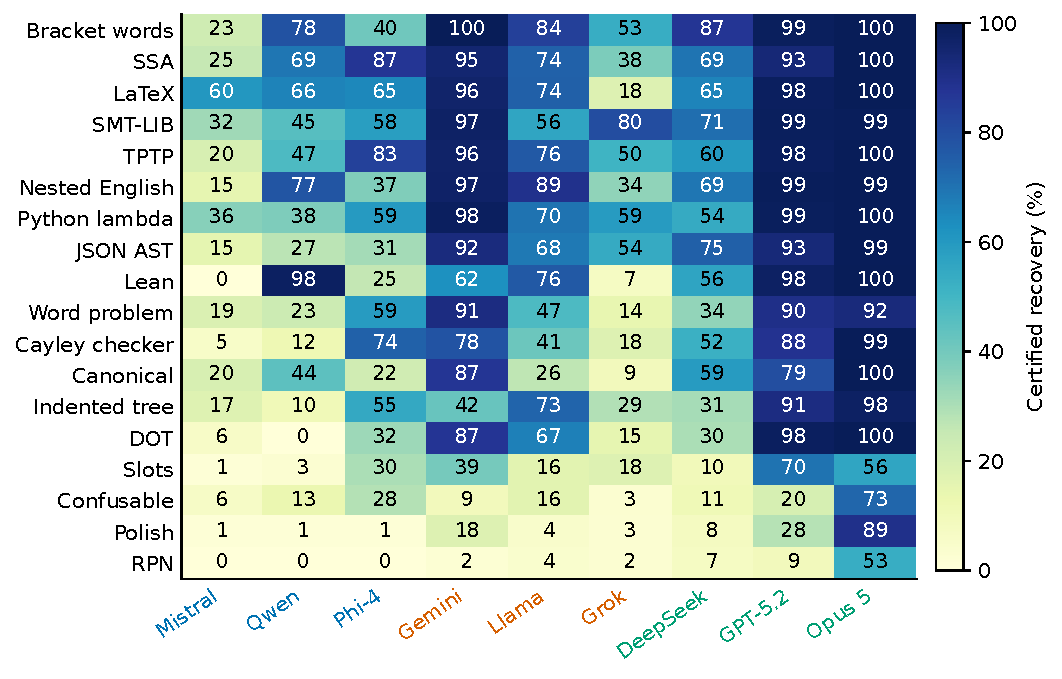
\includegraphics[width=\linewidth]{recovery-heatmap.pdf}
\caption{Main recovery by model and representation, with cells rounded to
integers. Rows are ordered by pooled recovery; model labels
are colored by descriptive tier (small: blue; medium: orange; frontier: green). The heatmap summarizes the fixed roster, not an
inference about model scale. Missing responses are excluded within each cell.}
\label{fig:heatmap}
\end{figure}

\subsection{The oracle distinguishes real semantic drift from coverage loss}

Across 81,000 main rows, there are 42,151 equivalent, 7,705 weaker, 1,087
stronger, and 7,576 incomparable answers. Fifteen mapped comparisons remain
unknown, 19,472 outputs are off catalogue/fragment, 2,925 are
unparseable/mapping failures, and 69 are content-filter loss. Thus the oracle
establishes strict semantic disagreement for 16,368 outputs, while separately
exposing substantial coverage loss (Figure~\ref{fig:outcomes}). Of the equivalent outputs, 2,281 map to a
different provably equivalent node; canonical-node matching alone would miss
those successes.

Confusable identifiers have a distinctive direction: 1,365/4,500 responses
(30.3\pct{}) are \emph{proven strictly weaker}, compared with 370/4,500
(8.2\pct{}) under LaTeX. Among these weaker outputs, 1,279/1,365 (93.7\pct{})
use fewer distinct variables than the source, versus 108/370 (29.2\pct{}) for
LaTeX. This concentration is consistent with variable identification; the
strict-weaker labels come from both certified implication directions, not from
that proxy. Equation~\ref{eq:merge} illustrates how preserving term shape while
losing a universal-variable distinction can enlarge the admissible-model class.

RPN shows a different failure pattern. Its broad off-fragment bucket is
2,434/4,500 (54.1\pct{}). Inspection of recorded mapping reasons identifies
2,340/4,500 (52.0\pct{}) as valid magma identities above order four; 94 other
outputs violate fragment restrictions. Many well-formed responses therefore
exceed the oracle's coverage. They cannot be certified by this oracle, but their
larger syntax \emph{does not prove inequivalence}. A translation evaluator needs
both semantic outcomes and coverage statistics to avoid turning this measurement
limitation into an unsupported error claim.

\begin{figure}[t]
\centering
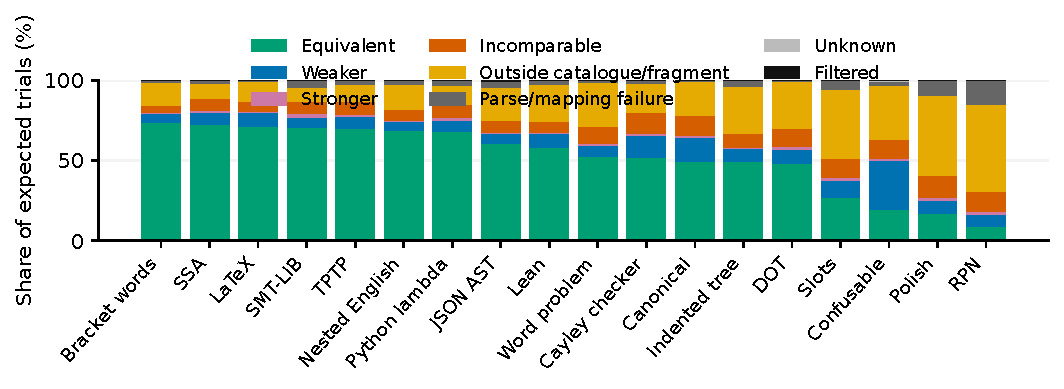
\includegraphics[width=\linewidth]{semantic-outcomes.pdf}
\caption{Semantic outcome composition across 4,500 expected main trials per
encoding. Proven weakening and strengthening are distinct from the large
outside-catalogue/fragment bucket, which does not establish inequivalence.
Filter losses and unknown comparisons are included, although small.}
\label{fig:outcomes}
\end{figure}

\subsection{Identifier changes can destroy recovery without causing refusals}

The naming study holds the operation AST, laws, models, and notation note fixed,
varying only a bijective variable-name tuple across six schemes
(Figure~\ref{fig:identifiers}). Accuracy drops from 64.4\pct{} on canonical letters to
3.1\pct{} on visually similar Latin/Cyrillic pairs. Among parseable incorrect
outputs, the fewer-variable proxy rises from 33.4\pct{} to 98.0\pct{}.
Unparseable rates stay at or below 3.0\pct{}. The effect is thus largely
expressed in parseable reconstructions, rather than absent answers.

\begin{figure}[t]
\centering
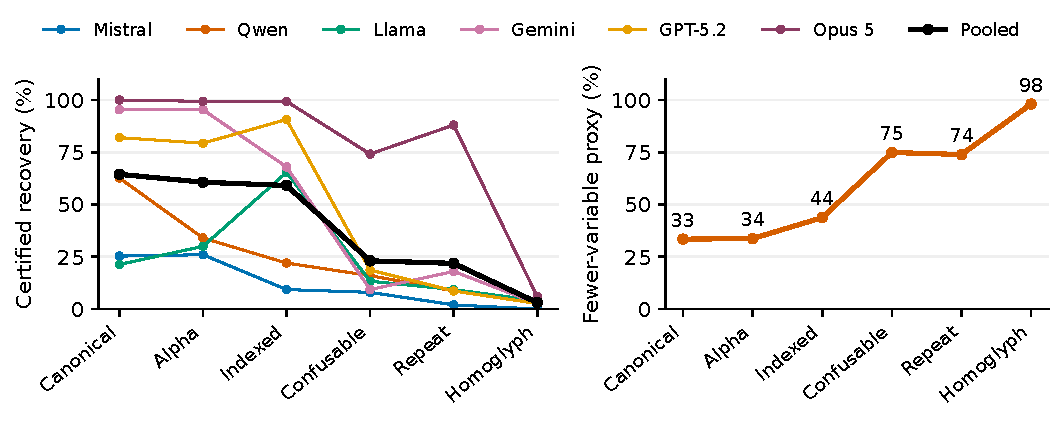
\includegraphics[width=\linewidth]{identifier-sensitivity.pdf}
\caption{Identifier study over six models and 150 laws. Left: recovery per
model and pooled over models, excluding 11 filtered responses. Right: fewer
distinct variables among incorrect outputs whose variables can be counted;
this is a proxy, not a proof of a pure variable-merge edit. Schemes are
categorical and not a calibrated numerical confusability scale. Exact
numerators, denominators, and code points appear in Appendix~\ref{app:naming}.}
\label{fig:identifiers}
\end{figure}

The aggregate trend is strong, but the proxy is not strictly monotone between
confusable and repeat schemes, and schemes are not a calibrated numerical
confusability scale. Opus goes from 100\pct{} on canonical letters to
6.0\pct{} on homoglyphs, despite retaining 74.1\pct{} on confusable ASCII and
88.0\pct{} on repeated-letter names. Indexed names improve Llama's recovery
from 21.3\pct{} to 65.3\pct{}, and GPT's from 82.0\pct{} to 90.7\pct{}.
Unusual or longer names are therefore not uniformly detrimental.

The homoglyph input is an injective AST-variable substitution, but cannot be
read back through the ASCII-oriented output parser. Requested outputs use
single lowercase letters; unsupported echoed glyphs can fail parsing. We report
this asymmetry rather than claiming the Unicode condition has the same
end-to-end validation as the seventeen alternate catalogues.

\subsection{Reading content helps selectively; extra context alone does not}

The note ablation crosses four models, four encodings, and four conditions over
150 laws. Conditions remove the note, retain it, pad it toward the generous
note's length, or supply detailed reading rules plus a micro-example. Generous
notes are 76--101 tokens; padded notes are within five tokens. The total is
9,600 fresh calls. Without any notation note, nested-English minus Polish
recovery remains positive for all four models: +64.0 points (Qwen), +90.0
(Gemini), +82.7 (GPT), and +43.3 (Opus). The main encoding contrast consequently
does not depend solely on the authored notes.

Reading content can nevertheless change the result dramatically. GPT's Polish
recovery moves from 34.0\pct{} with the current note to 93.3\pct{} with a
generous note; Opus's RPN moves from 49.3\pct{} to 94.0\pct{}. Both contrasts
survive within-model Holm correction. Table~\ref{tab:notes} shows selected
current, padded, and generous results. Against length-matched padding, the mean
gain across Polish/RPN cells is +27.8 points; across nested-English/LaTeX cells
it is $-0.2$ points. The padding-minus-current mean is $-2.2$ points across all
sixteen cells. These comparisons support a benefit from the \emph{specific
reading content}, not a general benefit from longer prompts.

\begin{table}[t]
\centering
\small
\caption{Selected notation-note interventions (recovery \pct). Current is the
main note; padded retains it with on-topic padding; generous adds explicit
reading rules and an example. Selection includes large gains and harmful
changes; the complete sixteen-cell table is in Appendix~\ref{app:notes}.}
\label{tab:notes}
\begin{tabular}{llrrr}
\toprule
Model & Encoding & Current & Padded & Generous \\
\midrule
GPT-5.2 & Polish & 34.0 & 30.0 & 93.3 \\
Opus 5 & RPN & 49.3 & 48.7 & 94.0 \\
Gemini 2.5 Flash & Polish & 19.3 & 28.7 & 68.7 \\
Qwen3 instruct & Polish & 0.7 & 0.7 & 15.3 \\
Qwen3 instruct & LaTeX & 72.7 & 69.3 & 57.3 \\
Gemini 2.5 Flash & LaTeX & 96.0 & 96.0 & 81.3 \\
\bottomrule
\end{tabular}
\end{table}

More explanation can also hurt. Generous versus current LaTeX notes reduce
Qwen by 15.3 points ($p_{\mathrm{Holm}}=0.0055$) and Gemini by 14.7
($p_{\mathrm{Holm}}=0.00010$). The intervention bundles rules and examples;
their separate effects are not identified, and padding is not guaranteed to be
cognitively inert. These findings argue for measured, notation-specific
documentation rather than maximal explanation.

\subsection{The canonical control reveals task-wording sensitivity}

Canonical infix shows the identity in the requested output notation, yet pooled
recovery is only 49.6\pct{}. This is a control for the \emph{configured recovery
task}, not an inherent model ceiling. The original output contract includes
``Do not restate the input,'' which can conflict with recovering a supplied
identity. A $2\times2$ framing probe adds an explicit anti-transformation rule,
removes the magma preamble, or applies both, on canonical and LaTeX inputs.
Seven models and 150 laws produce 8,400 calls.

\begin{table}[t]
\centering
\small
\caption{Canonical-control framing probe (recovery \pct). No transform adds an
explicit prohibition on deriving consequences, generalizing, or transforming
the identity. Bare removes the magma preamble. These are fresh 150-law baselines,
not the main 500-law control estimates.}
\label{tab:framing}
\begin{tabular}{lrrrr}
\toprule
Model & Baseline & No transform & Bare & Both \\
\midrule
Mistral Small & 18.7 & 65.3 & 19.3 & 69.3 \\
Qwen3 instruct & 50.0 & 75.3 & 36.0 & 80.0 \\
Phi-4 & 24.7 & 43.3 & 21.3 & 46.0 \\
Llama 4 Maverick & 25.3 & 68.7 & 16.7 & 77.3 \\
Grok 4.20 & 9.3 & 15.3 & 28.7 & 82.0 \\
Gemini 2.5 Flash & 83.3 & 98.0 & 92.0 & 95.3 \\
GPT-5.2 & 79.3 & 98.0 & 78.0 & 97.3 \\
\bottomrule
\end{tabular}
\end{table}

The sentence alone increases canonical recovery by 46.7 points for Mistral and
43.3 for Llama (differences from unrounded counts). Grok's largest change,
+72.7 points, requires \emph{both} edits; its sentence-alone gain is only
+6.0. Deleting the preamble alone is not significant for five of seven models.
The anti-transformation rule also improves LaTeX recovery: Mistral
60.0\pct{} to 78.0\pct{}, Qwen 78.0\pct{} to 96.7\pct{}, and Llama
74.7\pct{} to 94.7\pct{}, each adjusted $p<0.001$.
Improvement is therefore not specific to copying the canonical input.
The probe supports instruction sensitivity and is consistent with
over-transformation, but does not uniquely establish that psychological
mechanism. It also prevents interpreting the main results as intrinsic notation
difficulty independent of the recovery request.

\subsection{Repeated sampling limits fine-ranking interpretations}

On the 150 repeated laws, all three samples have the same reporting outcome in
18,704/24,300 triples (77.0\pct{}). Agreement refers to \emph{outcome labels},
including coverage failures, not necessarily identical reconstructed laws.
Across 162 model/representation cells, the range of recovery over three draws
has median 2.0 points, mean 2.9, 90th percentile 6.6, and maximum 20.0.
The broad 65.2-point main span is much larger than typical observed resampling
variation. However, nine of seventeen adjacent pooled gaps are smaller than the
median cell range. We emphasize broad groups rather than a best-format claim.

The range is a descriptive statistic from three draws on a smaller subset, not
a confidence interval or a universal two-point resolution threshold. Likewise,
overlap of nominal marginal intervals does not establish pairwise equivalence.
Confusable naming, slots, and RPN have the lowest outcome agreement
(64.6\pct{}, 67.3\pct{}, 68.6\pct{}); SSA and bracket words have the highest
(85.7\pct{}, 83.6\pct{}). Missing seed support and provider routing remain
sources of uncontrolled variation.

\section{Implications for verifiable coding and limitations}
\label{sec:discussion}

\paragraph{Specification preservation is a separate obligation.}
Within this domain, a certified weaker reconstruction admits magmas excluded by
the original identity. A later proof of that reconstruction cannot restore the
lost requirement. The right-projection witness in Equation~\ref{eq:merge} makes
this gap concrete. More generally, equivalence of specifications and correctness
of implementations against them are separate checks. We measure the former for
small equations, not the latter for generated programs.

\paragraph{Keep verdict direction and coverage in the interface.}
A Boolean pass/fail conflates opposite inclusion errors with out-of-coverage
answers. A preservation checker should expose intended-to-generated and
generated-to-intended evidence, together with an explicit uncertified outcome.
For supported pairs, weakening and strengthening have distinct downstream
consequences. For unsupported pairs, a stronger backend or human assessment is
needed before declaring equivalence or inequivalence. This is an implication of
the measurement, not a deployed tool evaluation.

\paragraph{Identifiers and instructions deserve evaluation.}
The confusable study motivates preserving a bijection between source and target
variable identities, checking co-reference structure, and considering existing
Unicode identifier-security mechanisms \citep{unicode2025security}.
The prompt probes show that reading examples and explicit preservation
instructions can help, but benefit is model/notation dependent. They were not
tested jointly, and extra documentation consumes prompt tokens. Neither a
discriminability linter nor an end-to-end repair pipeline is evaluated here.

\paragraph{Broader impact.}
Preservation checks could reduce false assurance when specifications are handled
by assistants. Conversely, the identifier distortions studied here could be
introduced deliberately to obscure variable distinctions. Treating an
uncertified output as a proven error, or a passed small-equation check as a
software-system guarantee, could also mislead users. We therefore report the
oracle boundary explicitly and evaluate no deployed security exploit.

\paragraph{Scope and measurement threats.}
The dataset comprises short single equations, with common algebraic notation
possibly present in pretraining; contamination is not quantified. The strata
overrepresent lower orders, and even reweighted estimates describe the
catalogue, not software specifications in general. Models are a fixed historical
API roster with unequal supported parameters and heterogeneous routing; tier
comparisons are descriptive. Follow-ups reused the 150-law subset and dispatched
tasks in condition blocks, leaving possible temporal/provider effects.
Notation notes and narrative scaffolding differ across encodings; the word
problem repeats caveats already in the frame. The Unicode naming schemes vary
script, visual similarity, length, and tokenization together.

The trusted measurement pipeline includes parsing, normalization, mapping,
render/inverse checks, and correct consumption of certified matrix statuses.
Some renderers/readers share helpers, so inverse agreement is not independent
formal verification. The catalogue is incomplete for arbitrary output syntax,
and strict extraction follows cleaning. Sixty-nine main filter losses are
concentrated in particular encodings; 499 main responses finish at the token
limit, so truncation is not absent. These limitations narrow the interpretation
of certified recovery, but do not negate the directly certified directional
relations for successfully mapped pairs.

\section{Conclusion}

Recovering the same formal identity from different deterministic encodings is
far from invariant under the evaluated protocol. The formal oracle adds more
than a correctness score: it detects thousands of strict inclusion errors,
including a concentration of weaker specifications under hostile identifiers,
while separately revealing outputs outside its coverage. Documentation and
preservation instructions recover substantial losses in selected settings;
repeat sampling discourages fine rankings. The resulting lesson for verifiable
coding is a measurable one: validate that the specification itself survives
model handling, report the direction of established drift, and make the boundary
of the semantic oracle explicit.

\section*{Reproducibility and use of language models}

An anonymous code-only supplement provides the oracle, converters,
experiment runners, grading, and a preparation entry point with embedded prompt
configuration. Saved responses and standalone analysis scripts are excluded.
Appendix~\ref{app:artifacts} distinguishes this supplement from the full research
record and gives setup instructions. No author-identifying repository link is included.
Final-row reported API costs total approximately \$103.92 for the 153,000-call
study; this is not a complete ledger of billed retries or pilot calls.
The design record precedes the main sweep according to project documentation,
but is not an immutable public preregistration. We disclose the model
substitution, corrected denominator, and exploratory extensions in
Appendix~\ref{app:deviations}.

LLMs are the evaluated systems. The earlier prose study additionally uses Qwen
to generate descriptions (Appendix~\ref{app:earlier}); those descriptions are
excluded from the main deterministic experiment. An LLM assistant was used to
draft and edit this manuscript and to check selected numerical claims against
stored artifacts. These steps did not generate new experimental results or
machine-checked proofs.

\bibliographystyle{plainnat}
\begin{thebibliography}{9}

\bibitem[Agarwal et~al.(2026)]{agarwal2026specgym}
Anmol Agarwal, Natalie Neamtu, Pranjal Aggarwal, Seungone Kim, Jannis Limperg,
Cedric Flamant, Kanna Shimizu, Bryan Parno, and Sean Welleck.
\newblock Verus-SpecGym: An Agentic Environment for Evaluating Specification
Autoformalization.
\newblock \emph{arXiv preprint arXiv:2605.26457}, 2026.
\newblock \url{https://arxiv.org/abs/2605.26457}.

\bibitem[Bolan et~al.(2025)]{bolan2025etp}
Matthew Bolan, Joachim Breitner, Jose Brox, Nicholas Carlini, Mario Carneiro,
Floris van Doorn, et~al.
\newblock The Equational Theories Project: Advancing Collaborative Mathematical
Research at Scale.
\newblock \emph{arXiv preprint arXiv:2512.07087}, 2025.
\newblock \url{https://arxiv.org/abs/2512.07087}.

\bibitem[Boucher and Anderson(2023)]{boucher2023trojan}
Nicholas Boucher and Ross Anderson.
\newblock Trojan Source: Invisible Vulnerabilities.
\newblock In \emph{32nd USENIX Security Symposium}, pages 6507--6524, 2023.
\newblock \url{https://www.usenix.org/conference/usenixsecurity23/presentation/boucher}.

\bibitem[Janota(2025)]{janota2025vampire}
Mikol\'{a}\v{s} Janota.
\newblock Experimental Results for Vampire on the Equational Theories Project.
\newblock \emph{arXiv preprint arXiv:2508.15856}, 2025.
\newblock \url{https://arxiv.org/abs/2508.15856}.

\bibitem[Murphy et~al.(2024)]{murphy2024geometry}
Logan Murphy, Kaiyu Yang, Jialiang Sun, Zhaoyu Li, Anima Anandkumar, and Xujie Si.
\newblock Autoformalizing Euclidean Geometry.
\newblock In \emph{International Conference on Machine Learning}, 2024.
\newblock \url{https://arxiv.org/abs/2405.17216}.

\bibitem[Sclar et~al.(2024)]{sclar2024format}
Melanie Sclar, Yejin Choi, Yulia Tsvetkov, and Alane Suhr.
\newblock Quantifying Language Models' Sensitivity to Spurious Features in
Prompt Design or: How I Learned to Start Worrying about Prompt Formatting.
\newblock In \emph{International Conference on Learning Representations}, 2024.
\newblock \url{https://arxiv.org/abs/2310.11324}.

\bibitem[Unicode Consortium(2025)]{unicode2025security}
Unicode Consortium.
\newblock Unicode Security Mechanisms.
\newblock Unicode Technical Standard \#39, revision 32, Unicode 17.0.0, 2025.
\newblock \url{https://www.unicode.org/reports/tr39/tr39-32.html}.

\bibitem[Wu et~al.(2022)]{wu2022autoformalization}
Yuhuai Wu, Albert Q. Jiang, Wenda Li, Markus N. Rabe, Charles Staats,
Mateja Jamnik, and Christian Szegedy.
\newblock Autoformalization with Large Language Models.
\newblock \emph{arXiv preprint arXiv:2205.12615}, 2022.
\newblock \url{https://arxiv.org/abs/2205.12615}.

\bibitem[Zheng et~al.(2022)]{zheng2022minif2f}
Kunhao Zheng, Jesse Michael Han, and Stanislas Polu.
\newblock miniF2F: A Cross-System Benchmark for Formal Olympiad-Level Mathematics.
\newblock In \emph{International Conference on Learning Representations}, 2022.
\newblock \url{https://arxiv.org/abs/2109.00110}.

\end{thebibliography}

\clearpage
\appendix

\section{Representation definitions and validation}
\label{app:representations}

Each catalogue stores \code{node}, \code{formal}, operation order,
distinct-variable count, and representation-specific text, with generator/style
and validation metadata. Canonical infix is taken from the formal field of an
alternate catalogue. The alternate renderings are:

\begin{enumerate}
\item \textbf{LaTeX}: infix \code{\diamond} and explicit parentheses.
\item \textbf{Lean}: universally quantified proposition over a type with a
\code{Magma} operation; the recovery body omits numbered law identifiers.
\item \textbf{Python lambda}: \code{lambda op, x, ...: lhs == rhs}, with nested
\code{op(a, b)} calls and explicit variable-parameter order.
\item \textbf{Python Cayley}: \code{def law(table)}, local
\code{n = len(table)}, and \code{all(... for x in range(n) ...)} with nested
\code{table[a][b]} lookups.
\item \textbf{Bracket-word text}: infix words \code{diamond}, \code{equals},
\code{open bracket}, and \code{close bracket}, with variable letters retained.
\item \textbf{Nested-English text}: recursive \code{the diamond of A and B}
phrases, with \code{equals} between sides.
\item \textbf{SSA}: post-order intermediate definitions, followed by equality of
side references; read-back expands definitions and checks their order.
\item \textbf{Slots}: a pair of nested binary lists; integer leaves are
first-appearance variable indices, preserving repeated-variable co-reference.
\item \textbf{RPN}: variable/postfix-operation tokens for both terms and a final
equality token; inverse reading simulates ordered stack consumption.
\item \textbf{Polish}: equality followed by two prefix terms; every binary
operation consumes two recursive terms.
\item \textbf{TPTP}: universally quantified first-order equality with uppercase
variable names and nested \code{op(A, B)} applications; formula name is generic.
\item \textbf{SMT-LIB}: uninterpreted sort/operation declarations plus a
universally quantified equality assertion using nested \code{(op a b)} terms.
\item \textbf{Indented tree}: one equality-rooted tree with two ordered children
and four-column indentation; branch markers carry traversal structure.
\item \textbf{DOT}: labeled equality/operation/variable nodes and ordered edges
in textual Graphviz source, using \code{ordering=out}.
\item \textbf{JSON AST}: one-key equality object with a two-term list; variables
are strings and operations are one-key diamond objects with ordered arguments.
\item \textbf{Confusable names}: canonical infix with a bijective renaming to
\code{l I ll lI Il II}.
\item \textbf{Word problem}: a fixed welding scenario and recursively nested
``part made by welding A to B'' descriptions, universally quantified over parts.
\end{enumerate}

Readers recover AST structure through format-specific parsing. Newer text and
structural readers recover canonical infix and invoke the oracle parser; Python
readers use Python's AST module. Confusable read-back is compared after
bijective normalization, other catalogue checks use exact structure. Builders
also check canonical source forms and, where implemented, distinct rendered
strings across nodes. Converter self-tests include malformed/corrupted
renderings. These mechanisms establish deterministic fidelity on the recorded
catalogue under the tested decoder, not independent correctness of arbitrary
external parsers or proof-assistant elaboration.

\section{Full endpoint configuration and model summaries}
\label{app:models}

\begin{table}[h]
\centering
\small
\caption{Historical OpenRouter endpoint IDs and parameters. All calls cap
output at 900 tokens. ``No field'' means the runner does not set a reasoning
argument. The tier is a project-defined category.}
\begin{tabularx}{\linewidth}{lXll}
\toprule
Tier & Endpoint & Reasoning & Temperature / seed \\
\midrule
Small & \nolinkurl{mistralai/mistral-small-3.2-24b-instruct} & No field & 0 / yes \\
Small & \nolinkurl{qwen/qwen3-30b-a3b-instruct-2507} & No field & 0 / yes \\
Small & \nolinkurl{microsoft/phi-4} & No field & 0 / yes \\
Medium & \nolinkurl{google/gemini-2.5-flash} & Disabled & 0 / yes \\
Medium & \nolinkurl{meta-llama/llama-4-maverick} & No field & 0 / yes \\
Medium & \nolinkurl{x-ai/grok-4.20} & Disabled & 0 / yes \\
Frontier & \nolinkurl{deepseek/deepseek-v3.2} & Disabled & 0 / yes \\
Frontier & \nolinkurl{openai/gpt-5.2} & Effort none & Omitted / yes \\
Frontier & \nolinkurl{anthropic/claude-opus-5} & Disabled & 0 / no \\
\bottomrule
\end{tabularx}
\end{table}

Supported seeds use \code{20260830 + k}; $k=0$ for the main and follow-up
calls, $k=1,2$ for extra repeats. The main task shuffle seed is 771 plus model
roster index. Sample seed is 20260830, repeat-subset selection seed 20260831.
Project documentation reports an 80-call reasoning preflight for the original
roster; DeepSeek's explicit disable setting was added after Kimi substitution.
Stored graded main/repeat rows record zero reasoning tokens. Explanatory ordinary
completion text is still possible.

\begin{table}[h]
\centering
\small
\caption{Recovery and strict-extraction scores (\pct), with all 9,000 expected
main calls per model in the denominator to make loss visible. These differ from
Equation~\ref{eq:recovery} for a model with excluded missing responses.
The canonical column uses all-answered cell accuracy.}
\begin{tabular}{lrrr}
\toprule
Model & Recovery / expected calls & Strict / expected calls & Canonical \\
\midrule
% BEGIN GENERATED MODEL SUMMARY
Phi-4 & 43.7 & 7.3 & 22.2 \\
Mistral Small & 16.7 & 16.6 & 19.8 \\
Qwen3 instruct & 36.2 & 36.2 & 44.4 \\
Gemini 2.5 Flash & 71.5 & 71.5 & 87.0 \\
Llama 4 Maverick & 53.5 & 48.7 & 26.2 \\
Grok 4.20 & 27.9 & 27.9 & 9.0 \\
Opus 5 & 91.3 & 82.5 & 100.0 \\
DeepSeek V3.2 & 47.0 & 46.9 & 58.8 \\
GPT-5.2 & 80.5 & 80.5 & 79.4 \\
% END GENERATED MODEL SUMMARY
\bottomrule
\end{tabular}
\end{table}

The strict gap is 36.4 points for Phi and 8.8 for Opus, rather than a single
outlier. Model tiers should not be interpreted as controlled scale effects.
Open-weight versus closed-weight recovery is likewise confounded with the
selected roster and tier distribution.

\section{Exact main counts and supplementary analyses}
\label{app:tables}

\begin{table}[ht]
\centering
\small
\caption{Main certified recovery (\pct), pooled over the fixed nine-model
roster. All-answered estimates exclude only missing-response outcomes. Common
uses 434 globally complete laws; post-stratified reweights eligible catalogue
orders. Fine rank differences should not be read as established pairwise
superiority. Exact counts and nominal intervals are in
Appendix~\ref{app:tables}.}
\label{tab:ranking}
\begin{tabular}{lrrr}
\toprule
Representation & All answered & Common & Post-stratified \\
\midrule
% BEGIN GENERATED RANKING
Bracket words & 73.7 & 73.6 & 73.3 \\
SSA & 72.2 & 72.4 & 71.7 \\
LaTeX & 71.4 & 71.6 & 73.0 \\
SMT-LIB & 70.7 & 70.8 & 69.7 \\
TPTP & 70.1 & 70.0 & 68.8 \\
Nested English & 68.5 & 69.1 & 67.0 \\
Python lambda & 67.9 & 67.8 & 67.2 \\
JSON AST & 61.2 & 62.6 & 59.9 \\
Lean & 58.1 & 58.5 & 61.1 \\
Word problem & 52.2 & 53.3 & 52.2 \\
Cayley checker & 51.9 & 52.5 & 51.2 \\
Canonical infix & 49.6 & 49.5 & 50.6 \\
Indented tree & 49.5 & 50.4 & 50.6 \\
DOT graph & 48.4 & 48.0 & 46.7 \\
Integer slots & 26.8 & 27.5 & 28.1 \\
Confusable names & 19.7 & 20.3 & 19.5 \\
Polish (prefix) & 16.9 & 17.5 & 16.7 \\
RPN (postfix) & 8.5 & 8.3 & 7.9 \\
% END GENERATED RANKING
\bottomrule
\end{tabular}
\end{table}

\begin{table}[h]
\centering
\small
\caption{Pooled main certified-equivalent numerators, nonmissing-response
denominators, and nominal Wilson 95\pct{} intervals. Intervals are descriptive
binomial summaries for the fixed roster and do not incorporate all dependence
between repeated laws or uncertainty over model selection.}
\begin{tabular}{lrrr}
\toprule
Representation & Equivalent & Nonmissing & 95\pct{} interval \\
\midrule
% BEGIN GENERATED EXACT COUNTS
Bracket words & 3317 & 4500 & 72.4--75.0 \\
SSA & 3249 & 4498 & 70.9--73.5 \\
LaTeX & 3213 & 4500 & 70.1--72.7 \\
SMT-LIB & 3182 & 4500 & 69.4--72.0 \\
TPTP & 3155 & 4500 & 68.8--71.4 \\
Nested English & 3081 & 4498 & 67.1--69.8 \\
Python lambda & 3057 & 4500 & 66.6--69.3 \\
JSON AST & 2729 & 4456 & 59.8--62.7 \\
Lean & 2613 & 4500 & 56.6--59.5 \\
Word problem & 2349 & 4500 & 50.7--53.7 \\
Cayley checker & 2334 & 4499 & 50.4--53.3 \\
Canonical infix & 2234 & 4500 & 48.2--51.1 \\
Indented tree & 2229 & 4500 & 48.1--51.0 \\
DOT graph & 2176 & 4500 & 46.9--49.8 \\
Integer slots & 1206 & 4500 & 25.5--28.1 \\
Confusable names & 882 & 4480 & 18.5--20.9 \\
Polish (prefix) & 761 & 4500 & 15.8--18.0 \\
RPN (postfix) & 384 & 4500 & 7.8--9.4 \\
% END GENERATED EXACT COUNTS
\bottomrule
\end{tabular}
\end{table}

\begin{table}[h]
\centering
\small
\caption{Main outcome counts over all 4,500 expected responses per encoding.
E/W/S/I are equivalent/weaker/stronger/incomparable; U is unknown;
O is off catalogue/fragment; P is unparseable/mapping failure; F is content
filter. No main output has the transport-error outcome.}
\begin{tabular}{lrrrrrrrr}
\toprule
Encoding & E & W & S & I & U & O & P & F \\
\midrule
% BEGIN GENERATED OUTCOMES
Bracket words & 3317 & 239 & 27 & 220 & 2 & 622 & 73 & 0 \\
SSA & 3249 & 345 & 51 & 333 & 0 & 425 & 95 & 2 \\
LaTeX & 3213 & 370 & 31 & 289 & 0 & 569 & 28 & 0 \\
SMT-LIB & 3182 & 267 & 124 & 318 & 2 & 412 & 195 & 0 \\
TPTP & 3155 & 335 & 58 & 354 & 0 & 485 & 113 & 0 \\
Nested English & 3081 & 270 & 34 & 299 & 1 & 700 & 113 & 2 \\
Python lambda & 3057 & 326 & 82 & 363 & 0 & 525 & 147 & 0 \\
JSON AST & 2729 & 271 & 33 & 348 & 0 & 911 & 164 & 44 \\
Lean & 2613 & 385 & 39 & 297 & 0 & 1045 & 121 & 0 \\
Word problem & 2349 & 331 & 46 & 478 & 3 & 1225 & 68 & 0 \\
Cayley checker & 2334 & 603 & 76 & 591 & 3 & 819 & 73 & 1 \\
Canonical infix & 2234 & 666 & 55 & 550 & 1 & 954 & 40 & 0 \\
Indented tree & 2229 & 350 & 38 & 393 & 0 & 1327 & 163 & 0 \\
DOT graph & 2176 & 385 & 76 & 501 & 0 & 1323 & 39 & 0 \\
Integer slots & 1206 & 482 & 92 & 530 & 0 & 1930 & 260 & 0 \\
Confusable names & 882 & 1365 & 53 & 537 & 2 & 1527 & 114 & 20 \\
Polish (prefix) & 761 & 376 & 85 & 612 & 1 & 2239 & 426 & 0 \\
RPN (postfix) & 384 & 339 & 87 & 563 & 0 & 2434 & 693 & 0 \\
% END GENERATED OUTCOMES
\bottomrule
\end{tabular}
\end{table}

Main filter losses by encoding are JSON AST 44, confusable names 20, SSA two,
nested-English two, and Cayley one. There are 499 length finishes, approximately
0.62\pct{} of main calls; a length finish may still yield an extracted answer.
The main/repeat total includes 99 filtered rows. Response loss is distinct from
the much larger coverage/parse-failure rate.

\paragraph{Difficulty covariates.}
An exploratory logistic model of correctness uses representation, order, and
tier, with standard errors clustered by source law: 80,931 responses,
500 clusters. The order coefficient is $-0.0169$ ($p=0.566$).
Representative coefficients relative to canonical are bracket words $+1.2263$,
SSA $+1.1414$, LaTeX $+1.0940$, slots $-1.1779$, confusable $-1.6308$,
Polish $-1.8445$, and RPN $-2.6883$. Frontier versus small tier is $+2.1907$;
this is a log-odds association, not directly comparable with percentage-point
intervention gains.

Depth 1/2/3/4 descriptive recovery is 55.4/58.8/51.0/45.4\pct{}; recovery
for 1--5 distinct variables is 55.6/52.8/51.4/52.4/52.4\pct{}.
Depth is not included in that fitted regression, so the depth association is
unadjusted. Equivalence-class size buckets unique/2--9/10+ have
54.0/54.2/51.0\pct{} recovery. These are exploratory descriptive comparisons,
not evidence that any covariate has no causal effect.

\section{Extraction and exact baseline frame}
\label{app:extraction}

Cleaning removes paired thinking/reasoning tags, selected stray tags,
typesetting spacing, math delimiters, and selected LaTeX text wrappers.
The extraction acceptance rule in the implemented grader is mapper status
different from \code{parse-failure}. This is broader than requiring successful
identity parsing: an outside-fragment or internal-error candidate can terminate
the ladder before a later valid candidate. Off-fragment includes constants,
unsupported relation symbols, or additional operations as well as valid
above-order-four identities. The reported results retain this original
implementation; no repaired-extractor experiment is presented.

The strict-extraction score requires \code{exact} after cleaning and oracle
normalization. It can therefore accept alternate operator notation or cleaned
presentation that does not literally follow the raw output contract. The
visible-CoT field is an extraction/presentation heuristic; it does not measure
hidden reasoning expenditure, and we do not use it to infer an internal
reasoning mechanism.

The following reproduces the baseline frame, with mathematical glyphs rendered
as TeX and placeholders shown explicitly. For canonical input, the note is:
``The operation is written $\diamond$ between its two arguments. Variables are
single lowercase letters. Grouping is shown by parentheses around each nested
operation.'' For confusable naming: ``The operation is written $\diamond$
between its two arguments. Variables are the identifiers; different identifiers
are different variables. Grouping is shown by parentheses.''

\begin{quote}
\small
A single identity that holds in a magma is written below. Recover the identity
itself.

The identity involves one binary operation and holds for all values of its
variables. The operation is on an arbitrary set: it is not assumed to be
associative or commutative, and there is no identity element.

\textit{[Notation note]}

Requirements:
\begin{itemize}
\item Output only the identity, on one line, in the form: left side = right side.
\item Write the operation as $\diamond$ and make every grouping explicit with
parentheses: write $x\op(y\op z)$ or $(x\op y)\op z$, never $x\op y\op z$.
\item Use single lowercase letters for variables; you may choose any letters.
\item Do not restate the input, do not name the identity, do not explain, and do
not add any other text.
\end{itemize}
\textit{[Rendered law]}
\end{quote}

The anti-transformation probe inserts: ``Write exactly the identity shown below.
Do not derive a consequence of it, do not generalise it, and do not transform it
in any way.'' The bare-frame manipulation removes the magma preamble paragraph
above. Both retains the inserted sentence and removes that paragraph.

\section{Complete notation-note ablation}
\label{app:notes}

\begin{table}[h]
\centering
\small
\caption{All sixteen model/encoding cells across four note conditions (recovery
\pct). Denominator is 150 except Opus generous nested-English 139, Opus generous
Polish 149, and Opus padded Polish 149, because filtered responses are excluded.
These exclusions matter for interpreting apparent ceiling scores.}
\begin{tabular}{llrrrr}
\toprule
Model & Encoding & None & Current & Padded & Generous \\
\midrule
% BEGIN GENERATED ABLATION
Qwen3 instruct & Nested English & 64.0 & 79.3 & 60.7 & 84.0 \\
Qwen3 instruct & Polish (prefix) & 0.0 & 0.7 & 0.7 & 15.3 \\
Qwen3 instruct & RPN (postfix) & 0.7 & 0.0 & 0.7 & 3.3 \\
Qwen3 instruct & LaTeX & 64.0 & 72.7 & 69.3 & 57.3 \\
Gemini 2.5 Flash & Nested English & 94.7 & 96.0 & 98.0 & 98.0 \\
Gemini 2.5 Flash & Polish (prefix) & 4.7 & 19.3 & 28.7 & 68.7 \\
Gemini 2.5 Flash & RPN (postfix) & 6.0 & 2.0 & 4.0 & 20.0 \\
Gemini 2.5 Flash & LaTeX & 90.7 & 96.0 & 96.0 & 81.3 \\
GPT-5.2 & Nested English & 93.3 & 98.7 & 98.7 & 98.7 \\
GPT-5.2 & Polish (prefix) & 10.7 & 34.0 & 30.0 & 93.3 \\
GPT-5.2 & RPN (postfix) & 8.0 & 4.7 & 8.7 & 34.7 \\
GPT-5.2 & LaTeX & 86.0 & 96.7 & 95.3 & 92.7 \\
Opus 5 & Nested English & 98.0 & 98.0 & 99.3 & 100.0 \\
Opus 5 & Polish (prefix) & 54.7 & 90.7 & 67.8 & 82.6 \\
Opus 5 & RPN (postfix) & 36.0 & 49.3 & 48.7 & 94.0 \\
Opus 5 & LaTeX & 100.0 & 100.0 & 96.0 & 100.0 \\
% END GENERATED ABLATION
\bottomrule
\end{tabular}
\end{table}

Per-encoding note lengths for current/padded/generous are nested-English
29/78/76, Polish 35/106/101, RPN 35/84/87, and LaTeX 27/76/76 tokens under
\code{cl100k_base}. Padded notes append complete on-topic sentences without
additional parsing instructions or imperatives. Generous notes specify argument
order and recursion/stack behavior, plus an example. For example, Polish
explains that leading equality consumes two terms and each operation consumes
two recursive terms; RPN explains pushes, two-value pops with left/right order,
and final equality. The ablation cannot separate reading instructions from
the included example.

The reported note tests compare none/padded/generous with current, paired by law
and corrected within model across representation/condition contrasts.
The descriptive generous-minus-padded mean is not itself a new family of
Holm-corrected significance tests. Thirteen responses are filtered and 207
finish at the output cap. Notes and raw responses are retained in the existing
artifacts.

\section{Exact notation notes and intervention text}
\label{app:promptnotes}

The following are the recorded main notes. Mathematical glyphs are typeset
rather than copied as Unicode characters; words and punctuation are unchanged.
All notes are constant across laws. Their \code{cl100k_base} lengths appear
in parentheses. The shared frame is in Appendix~\ref{app:extraction}.

\begin{description}
\item[\code{ascii_tree} (37 tokens)] Each $\diamond$ is one operation. Variables are the lowercase letters at the leaves. Grouping is shown by indentation: a node's two children are its arguments, the left one first.
\item[\code{confusable_vars} (29 tokens)] The operation is written $\diamond$ between its two arguments. Variables are the identifiers; different identifiers are different variables. Grouping is shown by parentheses.
\item[\code{etp_canonical} (28 tokens)] The operation is written $\diamond$ between its two arguments. Variables are single lowercase letters. Grouping is shown by parentheses around each nested operation.
\item[\code{graphviz} (35 tokens)] This is Graphviz DOT. Each $\diamond$ node is an operation. Variables are letters in node labels. A node's two out-edges are its arguments, left first.
\item[\code{json_ast} (31 tokens)] This is JSON. The operation is an object keyed $\diamond$ holding two arguments. Variables are the strings. Grouping is shown by how the objects nest.
\item[\code{latex} (27 tokens)] This is LaTeX. The operation is written \textbackslash{}diamond between its two arguments. Variables are single letters. Grouping is shown by parentheses.
\item[\code{lean} (31 tokens)] This is Lean. The operation is written $\diamond$ between its two arguments. Variables are the ones bound by the $\forall$. Grouping is shown by parentheses.
\item[\code{polish} (35 tokens)] The operation is $\diamond$, written before its two arguments. Variables are single lowercase letters. Grouping is shown by position: each $\diamond$ takes the two terms after it.
\item[\code{py_cayley_table} (35 tokens)] This is Python. The operation is the lookup table[a][b]. Variables are the names quantified in the comprehension. Grouping is shown by how the lookups nest.
\item[\code{py_lambda} (33 tokens)] This is Python. The operation is the call op(a, b). Variables are the lambda's parameters after op. Grouping is shown by how the calls nest.
\item[\code{rpn} (35 tokens)] The operation is $\diamond$, written after its two arguments. Variables are single lowercase letters. Grouping is shown by position: each $\diamond$ takes the two values before it.
\item[\code{slots} (39 tokens)] The operation is a two-element list. Variables are numbers, and equal numbers are the same variable. Grouping is shown by how the lists nest; the outermost list holds the two sides.
\item[\code{smtlib} (36 tokens)] This is SMT-LIB. The operation is the application (op a b). Variables are the names bound by the forall. Grouping is shown by how the applications nest.
\item[\code{ssa} (36 tokens)] The operation is written $\diamond$ between its two arguments. Variables are single lowercase letters; names starting with t are intermediate results. Grouping is shown by which results each line uses.
\item[\code{text} (30 tokens)] The operation is the word diamond between its two arguments. Variables are single lowercase letters. Grouping is shown by the words open bracket and close bracket.
\item[\code{text2} (29 tokens)] The operation is the phrase 'the diamond of A and B'. Variables are single lowercase letters. Grouping is shown by how those phrases nest.
\item[\code{tptp} (38 tokens)] This is TPTP. The operation is the term op(A, B). Variables are the upper-case names bound by the quantifier. Grouping is shown by how the terms nest.
\item[\code{word_problem} (32 tokens)] The operation is welding one part to another, in that order. Variables are the lowercase letters naming parts. Grouping is shown by which part each welding uses.
\end{description}

\paragraph{Generous notes.}
These replace, rather than append to, the corresponding current note.
\begin{description}
\item[\code{text2}] Each operation is the phrase 'the diamond of A and B', where A is the left argument and B the right. Variables are single lowercase letters. The phrases nest: in 'the diamond of x and the diamond of y and z', the left argument is x and the right argument is the whole inner phrase. Resolve the outermost phrase first, then each argument in turn.
\item[\code{polish}] This is Polish, or prefix, notation. The leading '=' takes the two terms that follow it as the left and right sides. Each '$\diamond$' takes the two terms that follow it as its left and right arguments. Variables are single lowercase letters. For example, '= $\diamond$ x y z' means (x $\diamond$ y) = z, because the '=' takes '$\diamond$ x y' as its first term and 'z' as its second. Every symbol consumes exactly two following terms.
\item[\code{rpn}] This is reverse Polish, or postfix, notation. Read left to right keeping a stack: a variable is pushed; a '$\diamond$' pops the two most recent values and pushes their combination, the earlier-pushed value being the left argument; the final '=' pops two values to form the two sides. Variables are single lowercase letters. For example, 'x y $\diamond$ z =' means (x $\diamond$ y) = z.
\item[\code{latex}] This is LaTeX. The operation is written \textbackslash{}diamond between its two arguments, so 'x \textbackslash{}diamond y' has x on the left and y on the right. Variables are single letters. Parentheses show grouping: 'x \textbackslash{}diamond (y \textbackslash{}diamond z)' has x on the left and the whole parenthesised expression on the right. Resolve the outermost operation first.
\end{description}

\paragraph{Padded notes.}
The recorded padded notes retain the current note and append the following
sentences in order, stopping when the target generous-note token count is
reached or when the next complete sentence would increase the absolute token
count difference. No sentence is truncated. Thus the selected suffix, not only
the token budget, is reproducible.
\begin{enumerate}
\item The operation combines exactly two arguments, and its result is again a value of the same kind.
\item The same operation is used at every point in the expression.
\item The identity is stated once, and it holds for every assignment of values to its variables.
\item Nothing in the expression below is abbreviated or elided.
\item The expression uses no convention beyond the one described above.
\item This is one identity, not a system of several.
\item The operation has no special cases, and the same reading applies throughout.
\end{enumerate}

The none condition removes the note; repeated blank lines left by that removal
are collapsed. The naming study uses the confusable note above for every
scheme, including canonical. The framing probe's inserted sentence and deleted
paragraph are specified in Appendix~\ref{app:extraction}.

\section{Identifier details and denominators}
\label{app:naming}

Homoglyph names are the six distinct strings with code points
\code{U+0061}, \code{U+0430}, \code{U+0065}, \code{U+0435},
\code{U+006F}, \code{U+043E}, respectively: Latin small a, Cyrillic small a,
Latin small e, Cyrillic small ie, Latin small o, Cyrillic small o. Code points
are given instead of relying on this paper's font to make differences visible.
The renderer substitutes names on AST variable leaves; distinct names remain
distinct in the input construction.

Pooled recovery numerator/denominator counts by scheme are canonical 580/900,
alpha 546/900, indexed 532/900, confusable 207/897, repeat 195/892, and
homoglyph 28/900. Proxy denominators in Figure~\ref{fig:identifiers} require an
incorrect extracted identity whose variables can be counted; unparseable and
filtered outputs do not enter them. Thus ``98\pct{}'' is not a claim about
all wrong calls. The same confusable notation note is used at every naming
level, including canonical; its baseline differs from the main canonical
condition's note.

\begin{table}[h]
\centering
\small
\caption{Identifier study: six models, 150 laws, 5,400 calls. Accuracy excludes
11 filtered responses; the fewer-variable proxy excludes wrong outputs whose
variables cannot be counted. Its counts are shown explicitly. Homoglyph names
pair Latin and Cyrillic letters; exact code points are in
Appendix~\ref{app:naming}.}
\label{tab:naming}
\begin{tabularx}{\linewidth}{lXrrr}
\toprule
Scheme & Identifiers & Recovery & Fewer vars. & Unparsed \\
\midrule
Canonical & \code{x y z w u v} & 64.4 & 33.4 (106/317) & 0.8 \\
Alpha & \code{a b c d e f} & 60.7 & 33.7 (119/353) & 0.6 \\
Indexed & \code{v1 v2 ... v6} & 59.1 & 43.8 (161/368) & 0.1 \\
Confusable & \code{l I ll lI Il II} & 23.1 & 74.9 (510/681) & 0.9 \\
Repeat & \code{l ll ... llllll} & 21.9 & 73.9 (496/671) & 3.0 \\
Homoglyph & Latin/Cyrillic $a,e,o$ pairs & 3.1 & 98.0 (853/870) & 2.0 \\
\bottomrule
\end{tabularx}
\end{table}

\section{Artifacts, execution flow, and deviations}
\label{app:artifacts}

\paragraph{Anonymous code supplement.}
The supplement contains only Python and shell source: oracle parsing, mapping,
matrix construction and comparison; deterministic converters and catalogue
builders; sampling, prompt rendering, API collection and grading; follow-up
runners; and earlier prose/implication experiment utilities. It contains no
Markdown, standalone analysis scripts, saved experiment responses, generated
catalogues, notebooks, credentials, repository history, local environments,
or paper/build artifacts. The historical data underlying the tables are not
bundled with this code-only release.

The root \code{prepare_experiment.py} embeds the original frame and all eighteen
notation notes. Its module documentation lists dependencies and execution
commands. After installing those dependencies and supplying the upstream ETP
\code{equations.txt} and \code{2024-11-10-outcomes.json.zip} through
\code{ETP_EQUATIONS}/\code{ETP_OUTCOMES} (or \code{ETP_ROOT}), run:
\begin{verbatim}
python3 prepare_experiment.py
cd semantic-diff-test
python3 run_experiment.py --smoke 2
\end{verbatim}
Preparation regenerates catalogue renderings, the local matrix, the sample,
and prompt files without calling model APIs. Collection requires
\code{OPENROUTER_API_KEY} and incurs API charges. Earlier experimental utilities
need their separately generated datasets and upstream inputs. The supplement
is prepared for upload with the submission, rather than represented as an
already published public repository.

\paragraph{Full research record.}
The following inventory describes the full project, including data and analysis
artifacts omitted from the anonymous supplement:

\begin{itemize}
\item \code{oracle/}: normalizer, mapper, matrix builder and comparison API/CLI;
local matrix and metadata for the historical outcomes snapshot.
\item \code{translate/<encoding>/}: deterministic converter, inverse reader,
catalogue builder and generated 4,694-row catalogue.
\item \code{semantic-diff-test/sample.json}, \code{frame.txt},
\code{prompts.json}, and per-encoding notes/templates/examples.
\item Per-encoding \code{raw-<model>.jsonl}: model/encoding/node/draw keys,
content, provider, finish, usage, retry count and timing.
\item \code{results/graded.json}: extracted identity, semantic outcome,
generated-node evidence where mapped, source-law covariates and run metadata;
\code{results/summary.json} and \code{tables.md}: derived analyses.
\item \code{ablation/}, \code{control_probe/}, \code{dose_confusable/}:
follow-up raw rows and summaries; \code{figures/}: generated raster plots.
\end{itemize}

Core parsing uses Python's standard library. API access uses the OpenAI SDK
against OpenRouter; analysis uses NumPy, SciPy, Matplotlib and \code{tiktoken},
with pandas/statsmodels for regression. The mapper requires ETP
\code{equations.txt}, selected by \code{ETP_EQUATIONS} or
\code{ETP_ROOT}; matrix construction additionally requires the snapshot outcomes
archive. Neither API credentials nor an author-specific external path is a
reproducibility requirement to disclose in a blind paper.

Once those inputs and alternate catalogues are available, the full research
workflow is as follows; \code{analyze.py} belongs to the original project and
is excluded from the code-only supplement:
\begin{verbatim}
cd semantic-diff-test
python3 build_sample.py
python3 render_prompts.py
python3 run_experiment.py --phase main
python3 run_experiment.py --phase repeat
python3 grade.py
python3 analyze.py
python3 ablate_notes.py --run --report
python3 probe_control.py --run --report
python3 dose_confusable.py --run --report
\end{verbatim}
Commands launching sweeps require an API key and incur spend. Regrading and
analysis can instead use stored responses. The numerical checker targets
selected fields in the Markdown analysis, not every sentence of this paper.
No byte-identical rerun guarantee is implied for dynamic API providers.

Main checkpoints flush each completed row and check headers pinning model,
temperature, output cap, reasoning, sample seed/count, and shared-frame hash.
They do not pin all individual note/rendering hashes or the entire node list;
follow-up checkpoints lack those identity headers. Error rows can be replaced
by recovered calls, but deduplication otherwise keeps the first accepted keyed
row rather than a general last-row rule. Artifact preservation is therefore
important; changing prompts and resuming in place is not fully protected.

Final-row costs are main/repeat \$79.6470, four-condition note ablation
\$18.7839, framing \$1.3787, naming \$4.1103, approximately \$103.92 total.
This accounting excludes the abandoned model, earlier experiments, and any
billed discarded retry responses not preserved in returned row costs.

\subsection{Changes to the recorded design}
\label{app:deviations}

The recorded main design initially used \code{moonshotai/kimi-k2} for an
open-weight frontier slot. Provider rate limiting prompted replacement with
\code{deepseek/deepseek-v3.2}. The 533 partial Kimi rows are retained separately
and excluded from all study tables. Its recorded final-response costs total
approximately \$0.1373.

The original denominator excluded unparseable and off-catalogue answers. We
instead count them as unsuccessful certification, excluding only missing
response outcomes; the original globally-gradeable rule yields zero common
laws, whereas the implemented nonmissing rule yields 434. The original cap of
400 tokens was increased to 900; concurrency also changed from early estimates.
Paired tests use the common subset, while pooled headline estimates use all
nonmissing responses. The note ablation, later padded-note addition, framing
probe, identifier study, and additional covariate analyses are follow-ups to the
main observations. The design record is not claimed to be an immutable external
preregistration.

\section{Earlier exploratory studies}
\label{app:earlier}

These studies motivated the controlled recovery design but are not part of its
153,000-call ledger and do not provide independent replication of its effects.

\paragraph{Generated-English round trip.}
Qwen \code{qwen/qwen3-30b-a3b} generated descriptions for the 4,694 laws,
with 4,612 usable descriptions, 42 empty and 40 failed results, at recorded
cost \$2.7783. The same endpoint reconstructed from descriptions alone;
of 4,694 output rows, 3,770 had usable answers. Semantic labels were 3,129
equivalent, 206 weaker, 48 stronger, 214 incomparable; 173 were unresolved and
924 lacked usable reconstructions. Equivalent share was 87.0\pct{} of
resolved, 83.0\pct{} of answered, and 66.7\pct{} of all catalogue rows.
Recorded reverse cost was \$5.7867. This joint forward/reverse measurement
confounds prose loss with reconstruction and has a substantial empty-answer
tail. Its model/settings differ from the later instruct-2507 condition, and
reasoning headroom differs from the controlled recovery protocol.

\paragraph{Implication judgment.}
A balanced sample of 250 certified true/false ordered pairs, seed 20260827,
was presented in ETP, LaTeX, Lean, generated English, Python lambda and Cayley
form to Mistral Small, Gemini 2.5 Flash and Opus 4.5. ATP time from a
2025-08-11 Vampire run provided difficulty signals, contextualized by
\citet{janota2025vampire}; truth labels used the historical oracle matrix.
The dataset used 298 distinct equations, excluded nodes 1/2, required usable
representations, and capped node reuse at four. Models answered TRUE/FALSE with
brief justification and confidence.

There were 4,500 judgments, no unrecovered transport failures, and 4,426 scored
answers; 74 lacked parsed verdicts, attributed to truncation and excluded from
accuracy. Overall accuracies were 55.9/75.8/82.4\pct{} for the three models,
recorded cost \$23.17. On the global 197-pair common subset, all six notations
agreed in 43.1/40.6/79.7\pct{} of items. Model-specific omnibus p-values were
0.000389/0.0210/0.0446; only three of 45 pairwise contrasts survived
within-model Holm adjustment. There was no same-prompt repeat arm, so agreement
does not isolate notation effects from resampling.

Generated English pooled accuracy was 68.0\pct{}, versus Cayley 74.6\pct{}.
Faithful-description subsets improved Gemini/Opus by about ten points,
indicating a prose-fidelity confound. These English results concern model-written
descriptions, unlike the deterministic English encodings in the main study.
Signal-detection analysis found substantial answer-bias shifts: Mistral favored
FALSE and Opus favored TRUE. This stage addresses reasoning/criterion effects
over an implication question, not recovery of a single law.

\clearpage
% Official NeurIPS 2026 checklist; questions and guidelines unchanged.
% Source: https://media.neurips.cc/Conferences/NeurIPS2026/Formatting_Instructions_For_NeurIPS_2026.zip
\section*{NeurIPS Paper Checklist}




\begin{enumerate}

\item {\bf Claims}
    \item[] Question: Do the main claims made in the abstract and introduction accurately reflect the paper's contributions and scope?
    \item[] Answer: \answerYes{}
    \item[] Justification: Sections~\ref{sec:intro}--\ref{sec:results} restrict claims to the configured recovery task and distinguish certified semantic disagreement from oracle coverage loss.
    \item[] Guidelines:
    \begin{itemize}
        \item The answer \answerNA{} means that the abstract and introduction do not include the claims made in the paper.
        \item The abstract and/or introduction should clearly state the claims made, including the contributions made in the paper and important assumptions and limitations. A \answerNo{} or \answerNA{} answer to this question will not be perceived well by the reviewers. 
        \item The claims made should match theoretical and experimental results, and reflect how much the results can be expected to generalize to other settings. 
        \item It is fine to include aspirational goals as motivation as long as it is clear that these goals are not attained by the paper. 
    \end{itemize}

\item {\bf Limitations}
    \item[] Question: Does the paper discuss the limitations of the work performed by the authors?
    \item[] Answer: \answerYes{}
    \item[] Justification: Section~\ref{sec:discussion} and Appendices~\ref{app:extraction} and~\ref{app:deviations} discuss scope, prompt ambiguity, parser limits, API variability, and exploratory follow-ups.
    \item[] Guidelines:
    \begin{itemize}
        \item The answer \answerNA{} means that the paper has no limitation while the answer \answerNo{} means that the paper has limitations, but those are not discussed in the paper. 
        \item The authors are encouraged to create a separate ``Limitations'' section in their paper.
        \item The paper should point out any strong assumptions and how robust the results are to violations of these assumptions (e.g., independence assumptions, noiseless settings, model well-specification, asymptotic approximations only holding locally). The authors should reflect on how these assumptions might be violated in practice and what the implications would be.
        \item The authors should reflect on the scope of the claims made, e.g., if the approach was only tested on a few datasets or with a few runs. In general, empirical results often depend on implicit assumptions, which should be articulated.
        \item The authors should reflect on the factors that influence the performance of the approach. For example, a facial recognition algorithm may perform poorly when image resolution is low or images are taken in low lighting. Or a speech-to-text system might not be used reliably to provide closed captions for online lectures because it fails to handle technical jargon.
        \item The authors should discuss the computational efficiency of the proposed algorithms and how they scale with dataset size.
        \item If applicable, the authors should discuss possible limitations of their approach to address problems of privacy and fairness.
        \item While the authors might fear that complete honesty about limitations might be used by reviewers as grounds for rejection, a worse outcome might be that reviewers discover limitations that aren't acknowledged in the paper. The authors should use their best judgment and recognize that individual actions in favor of transparency play an important role in developing norms that preserve the integrity of the community. Reviewers will be specifically instructed to not penalize honesty concerning limitations.
    \end{itemize}

\item {\bf Theory assumptions and proofs}
    \item[] Question: For each theoretical result, does the paper provide the full set of assumptions and a complete (and correct) proof?
    \item[] Answer: \answerYes{}
    \item[] Justification: Section~\ref{sec:measurement} states universal quantification and proves the variable-identification implication using induced assignments, with an explicit counterexample establishing strictness for Equation~\ref{eq:merge}.
    \item[] Guidelines:
    \begin{itemize}
        \item The answer \answerNA{} means that the paper does not include theoretical results. 
        \item All the theorems, formulas, and proofs in the paper should be numbered and cross-referenced.
        \item All assumptions should be clearly stated or referenced in the statement of any theorems.
        \item The proofs can either appear in the main paper or the supplemental material, but if they appear in the supplemental material, the authors are encouraged to provide a short proof sketch to provide intuition. 
        \item Inversely, any informal proof provided in the core of the paper should be complemented by formal proofs provided in appendix or supplemental material.
        \item Theorems and Lemmas that the proof relies upon should be properly referenced. 
    \end{itemize}

    \item {\bf Experimental result reproducibility}
    \item[] Question: Does the paper fully disclose all the information needed to reproduce the main experimental results of the paper to the extent that it affects the main claims and/or conclusions of the paper (regardless of whether the code and data are provided or not)?
    \item[] Answer: \answerYes{}
    \item[] Justification: Sections~\ref{sec:measurement} and~\ref{sec:design}, and Appendices~\ref{app:representations}, \ref{app:models}, \ref{app:extraction}, and~\ref{app:promptnotes}, specify the oracle snapshot, sampling, encodings, parameters, extraction, frame, and exact notes. Hosted-model variation prevents a byte-identical new API run; the artifacts described in Appendix~\ref{app:artifacts} support verification from saved responses.
    \item[] Guidelines:
    \begin{itemize}
        \item The answer \answerNA{} means that the paper does not include experiments.
        \item If the paper includes experiments, a \answerNo{} answer to this question will not be perceived well by the reviewers: Making the paper reproducible is important, regardless of whether the code and data are provided or not.
        \item If the contribution is a dataset and\slash or model, the authors should describe the steps taken to make their results reproducible or verifiable. 
        \item Depending on the contribution, reproducibility can be accomplished in various ways. For example, if the contribution is a novel architecture, describing the architecture fully might suffice, or if the contribution is a specific model and empirical evaluation, it may be necessary to either make it possible for others to replicate the model with the same dataset, or provide access to the model. In general. releasing code and data is often one good way to accomplish this, but reproducibility can also be provided via detailed instructions for how to replicate the results, access to a hosted model (e.g., in the case of a large language model), releasing of a model checkpoint, or other means that are appropriate to the research performed.
        \item While NeurIPS does not require releasing code, the conference does require all submissions to provide some reasonable avenue for reproducibility, which may depend on the nature of the contribution. For example
        \begin{enumerate}
            \item If the contribution is primarily a new algorithm, the paper should make it clear how to reproduce that algorithm.
            \item If the contribution is primarily a new model architecture, the paper should describe the architecture clearly and fully.
            \item If the contribution is a new model (e.g., a large language model), then there should either be a way to access this model for reproducing the results or a way to reproduce the model (e.g., with an open-source dataset or instructions for how to construct the dataset).
            \item We recognize that reproducibility may be tricky in some cases, in which case authors are welcome to describe the particular way they provide for reproducibility. In the case of closed-source models, it may be that access to the model is limited in some way (e.g., to registered users), but it should be possible for other researchers to have some path to reproducing or verifying the results.
        \end{enumerate}
    \end{itemize}


\item {\bf Open access to data and code}
    \item[] Question: Does the paper provide open access to the data and code, with sufficient instructions to faithfully reproduce the main experimental results, as described in supplemental material?
    \item[] Answer: \answerNo{}
    \item[] Justification: An anonymous code-only supplement is prepared for submission, with setup instructions in Appendix~\ref{app:artifacts}. Saved experimental data and standalone analyses are excluded, and no public download or completed upload is claimed; hence this is not full open access to both code and data.
    \item[] Guidelines:
    \begin{itemize}
        \item The answer \answerNA{} means that paper does not include experiments requiring code.
        \item Please see the NeurIPS code and data submission guidelines (\url{https://neurips.cc/public/guides/CodeSubmissionPolicy}) for more details.
        \item While we encourage the release of code and data, we understand that this might not be possible, so \answerNo{} is an acceptable answer. Papers cannot be rejected simply for not including code, unless this is central to the contribution (e.g., for a new open-source benchmark).
        \item The instructions should contain the exact command and environment needed to run to reproduce the results. See the NeurIPS code and data submission guidelines (\url{https://neurips.cc/public/guides/CodeSubmissionPolicy}) for more details.
        \item The authors should provide instructions on data access and preparation, including how to access the raw data, preprocessed data, intermediate data, and generated data, etc.
        \item The authors should provide scripts to reproduce all experimental results for the new proposed method and baselines. If only a subset of experiments are reproducible, they should state which ones are omitted from the script and why.
        \item At submission time, to preserve anonymity, the authors should release anonymized versions (if applicable).
        \item Providing as much information as possible in supplemental material (appended to the paper) is recommended, but including URLs to data and code is permitted.
    \end{itemize}


\item {\bf Experimental setting/details}
    \item[] Question: Does the paper specify all the training and test details (e.g., data splits, hyperparameters, how they were chosen, type of optimizer) necessary to understand the results?
    \item[] Answer: \answerYes{}
    \item[] Justification: Section~\ref{sec:design} and Appendices~\ref{app:models} and~\ref{app:promptnotes} specify inference parameters, sampling, prompts, and interventions; no model training is performed.
    \item[] Guidelines:
    \begin{itemize}
        \item The answer \answerNA{} means that the paper does not include experiments.
        \item The experimental setting should be presented in the core of the paper to a level of detail that is necessary to appreciate the results and make sense of them.
        \item The full details can be provided either with the code, in appendix, or as supplemental material.
    \end{itemize}

\item {\bf Experiment statistical significance}
    \item[] Question: Does the paper report error bars suitably and correctly defined or other appropriate information about the statistical significance of the experiments?
    \item[] Answer: \answerYes{}
    \item[] Justification: Sections~\ref{sec:design} and~\ref{sec:results} report paired tests, Holm corrections, and repeated-sampling variability. Appendix~\ref{app:tables} explains nominal Wilson intervals and dependence limitations; exploratory naming and padding comparisons are not claimed as independently confirmed causal effects.
    \item[] Guidelines:
    \begin{itemize}
        \item The answer \answerNA{} means that the paper does not include experiments.
        \item The authors should answer \answerYes{} if the results are accompanied by error bars, confidence intervals, or statistical significance tests, at least for the experiments that support the main claims of the paper.
        \item The factors of variability that the error bars are capturing should be clearly stated (for example, train/test split, initialization, random drawing of some parameter, or overall run with given experimental conditions).
        \item The method for calculating the error bars should be explained (closed form formula, call to a library function, bootstrap, etc.)
        \item The assumptions made should be given (e.g., Normally distributed errors).
        \item It should be clear whether the error bar is the standard deviation or the standard error of the mean.
        \item It is OK to report 1-sigma error bars, but one should state it. The authors should preferably report a 2-sigma error bar than state that they have a 96\% CI, if the hypothesis of Normality of errors is not verified.
        \item For asymmetric distributions, the authors should be careful not to show in tables or figures symmetric error bars that would yield results that are out of range (e.g., negative error rates).
        \item If error bars are reported in tables or plots, the authors should explain in the text how they were calculated and reference the corresponding figures or tables in the text.
    \end{itemize}

\item {\bf Experiments compute resources}
    \item[] Question: For each experiment, does the paper provide sufficient information on the computer resources (type of compute workers, memory, time of execution) needed to reproduce the experiments?
    \item[] Answer: \answerNo{}
    \item[] Justification: Appendix~\ref{app:artifacts} reports API call counts, costs, providers, and output caps, but provider hardware, energy, and discarded-retry compute are unavailable, and a complete local-resource inventory is not documented.
    \item[] Guidelines:
    \begin{itemize}
        \item The answer \answerNA{} means that the paper does not include experiments.
        \item The paper should indicate the type of compute workers CPU or GPU, internal cluster, or cloud provider, including relevant memory and storage.
        \item The paper should provide the amount of compute required for each of the individual experimental runs as well as estimate the total compute. 
        \item The paper should disclose whether the full research project required more compute than the experiments reported in the paper (e.g., preliminary or failed experiments that didn't make it into the paper). 
    \end{itemize}
    
\item {\bf Code of ethics}
    \item[] Question: Does the research conducted in the paper conform, in every respect, with the NeurIPS Code of Ethics \url{https://neurips.cc/public/EthicsGuidelines}?
    \item[] Answer: \answerYes{}
    \item[] Justification: The experiments use synthetic mathematical identities, without human participants or personal data. Prior work is credited and coverage limits, protocol changes, and remaining artifact-access and licensing-documentation gaps are disclosed.
    \item[] Guidelines:
    \begin{itemize}
        \item The answer \answerNA{} means that the authors have not reviewed the NeurIPS Code of Ethics.
        \item If the authors answer \answerNo, they should explain the special circumstances that require a deviation from the Code of Ethics.
        \item The authors should make sure to preserve anonymity (e.g., if there is a special consideration due to laws or regulations in their jurisdiction).
    \end{itemize}


\item {\bf Broader impacts}
    \item[] Question: Does the paper discuss both potential positive societal impacts and negative societal impacts of the work performed?
    \item[] Answer: \answerYes{}
    \item[] Justification: Section~\ref{sec:discussion} discusses potential reductions in false assurance, deliberate identifier distortion, and misleading extrapolation beyond the oracle domain.
    \item[] Guidelines:
    \begin{itemize}
        \item The answer \answerNA{} means that there is no societal impact of the work performed.
        \item If the authors answer \answerNA{} or \answerNo, they should explain why their work has no societal impact or why the paper does not address societal impact.
        \item Examples of negative societal impacts include potential malicious or unintended uses (e.g., disinformation, generating fake profiles, surveillance), fairness considerations (e.g., deployment of technologies that could make decisions that unfairly impact specific groups), privacy considerations, and security considerations.
        \item The conference expects that many papers will be foundational research and not tied to particular applications, let alone deployments. However, if there is a direct path to any negative applications, the authors should point it out. For example, it is legitimate to point out that an improvement in the quality of generative models could be used to generate Deepfakes for disinformation. On the other hand, it is not needed to point out that a generic algorithm for optimizing neural networks could enable people to train models that generate Deepfakes faster.
        \item The authors should consider possible harms that could arise when the technology is being used as intended and functioning correctly, harms that could arise when the technology is being used as intended but gives incorrect results, and harms following from (intentional or unintentional) misuse of the technology.
        \item If there are negative societal impacts, the authors could also discuss possible mitigation strategies (e.g., gated release of models, providing defenses in addition to attacks, mechanisms for monitoring misuse, mechanisms to monitor how a system learns from feedback over time, improving the efficiency and accessibility of ML).
    \end{itemize}
    
\item {\bf Safeguards}
    \item[] Question: Does the paper describe safeguards that have been put in place for responsible release of data or models that have a high risk for misuse (e.g., pre-trained language models, image generators, or scraped datasets)?
    \item[] Answer: \answerNA{}
    \item[] Justification: The paper releases no trained model, sensitive scraped dataset, or demonstrated deployed exploit; evaluated inputs are small mathematical identities.
    \item[] Guidelines:
    \begin{itemize}
        \item The answer \answerNA{} means that the paper poses no such risks.
        \item Released models that have a high risk for misuse or dual-use should be released with necessary safeguards to allow for controlled use of the model, for example by requiring that users adhere to usage guidelines or restrictions to access the model or implementing safety filters. 
        \item Datasets that have been scraped from the Internet could pose safety risks. The authors should describe how they avoided releasing unsafe images.
        \item We recognize that providing effective safeguards is challenging, and many papers do not require this, but we encourage authors to take this into account and make a best faith effort.
    \end{itemize}

\item {\bf Licenses for existing assets}
    \item[] Question: Are the creators or original owners of assets (e.g., code, data, models), used in the paper, properly credited and are the license and terms of use explicitly mentioned and properly respected?
    \item[] Answer: \answerNo{}
    \item[] Justification: ETP and prior work are credited, and snapshot/model versions are identified, but the research records do not establish a complete license and API-terms inventory for every asset. No completed audit is claimed.
    \item[] Guidelines:
    \begin{itemize}
        \item The answer \answerNA{} means that the paper does not use existing assets.
        \item The authors should cite the original paper that produced the code package or dataset.
        \item The authors should state which version of the asset is used and, if possible, include a URL.
        \item The name of the license (e.g., CC-BY 4.0) should be included for each asset.
        \item For scraped data from a particular source (e.g., website), the copyright and terms of service of that source should be provided.
        \item If assets are released, the license, copyright information, and terms of use in the package should be provided. For popular datasets, \url{paperswithcode.com/datasets} has curated licenses for some datasets. Their licensing guide can help determine the license of a dataset.
        \item For existing datasets that are re-packaged, both the original license and the license of the derived asset (if it has changed) should be provided.
        \item If this information is not available online, the authors are encouraged to reach out to the asset's creators.
    \end{itemize}

\item {\bf New assets}
    \item[] Question: Are new assets introduced in the paper well documented and is the documentation provided alongside the assets?
    \item[] Answer: \answerNo{}
    \item[] Justification: The anonymous code supplement includes embedded prompt configuration and a documented preparation entry point (Appendix~\ref{app:artifacts}). Derived catalogues and saved results are excluded, and a finalized release license for the complete derived assets is not provided.
    \item[] Guidelines:
    \begin{itemize}
        \item The answer \answerNA{} means that the paper does not release new assets.
        \item Researchers should communicate the details of the dataset\slash code\slash model as part of their submissions via structured templates. This includes details about training, license, limitations, etc. 
        \item The paper should discuss whether and how consent was obtained from people whose asset is used.
        \item At submission time, remember to anonymize your assets (if applicable). You can either create an anonymized URL or include an anonymized zip file.
    \end{itemize}

\item {\bf Crowdsourcing and research with human subjects}
    \item[] Question: For crowdsourcing experiments and research with human subjects, does the paper include the full text of instructions given to participants and screenshots, if applicable, as well as details about compensation (if any)? 
    \item[] Answer: \answerNA{}
    \item[] Justification: No crowdsourcing or experiments with human subjects are reported.
    \item[] Guidelines:
    \begin{itemize}
        \item The answer \answerNA{} means that the paper does not involve crowdsourcing nor research with human subjects.
        \item Including this information in the supplemental material is fine, but if the main contribution of the paper involves human subjects, then as much detail as possible should be included in the main paper. 
        \item According to the NeurIPS Code of Ethics, workers involved in data collection, curation, or other labor should be paid at least the minimum wage in the country of the data collector. 
    \end{itemize}

\item {\bf Institutional review board (IRB) approvals or equivalent for research with human subjects}
    \item[] Question: Does the paper describe potential risks incurred by study participants, whether such risks were disclosed to the subjects, and whether Institutional Review Board (IRB) approvals (or an equivalent approval/review based on the requirements of your country or institution) were obtained?
    \item[] Answer: \answerNA{}
    \item[] Justification: No human participants are involved in the reported experiments.
    \item[] Guidelines:
    \begin{itemize}
        \item The answer \answerNA{} means that the paper does not involve crowdsourcing nor research with human subjects.
        \item Depending on the country in which research is conducted, IRB approval (or equivalent) may be required for any human subjects research. If you obtained IRB approval, you should clearly state this in the paper. 
        \item We recognize that the procedures for this may vary significantly between institutions and locations, and we expect authors to adhere to the NeurIPS Code of Ethics and the guidelines for their institution. 
        \item For initial submissions, do not include any information that would break anonymity (if applicable), such as the institution conducting the review.
    \end{itemize}

\item {\bf Declaration of LLM usage}
    \item[] Question: Does the paper describe the usage of LLMs if it is an important, original, or non-standard component of the core methods in this research? Note that if the LLM is used only for writing, editing, or formatting purposes and does \emph{not} impact the core methodology, scientific rigor, or originality of the research, declaration is not required.
    %this research? 
    \item[] Answer: \answerYes{}
    \item[] Justification: Section~\ref{sec:design} specifies the evaluated LLMs and calls; Appendix~\ref{app:earlier} describes the separate model-generated prose study. The reproducibility disclosure describes manuscript assistance.
    \item[] Guidelines:
    \begin{itemize}
        \item The answer \answerNA{} means that the core method development in this research does not involve LLMs as any important, original, or non-standard components.
        \item Please refer to our LLM policy in the NeurIPS handbook for what should or should not be described.
    \end{itemize}

\end{enumerate}

\end{document}
